% Generated by pysimcount.pfchilds -- do not edit; regenerate instead.
% figure: main-total-all-formulas -- Every formula, X-Y-Z grouping, total gates vs n (cf. Childs et al. 2018 Fig. 3 right)
% source: ../np-main/aggregate.json + ../np-main-n9/seed{seed}, ../np-main-n11/seed{seed} (seeds [1, 2, 3, 4, 5, 6, 7, 8, 9, 10]); run commits: 01d3c275ceae2840002bd1aaea68f59b987c4975, e42ff29056ad9ea7fc7c9899fab334903e42e3e3
% metric=total kind=xyz merged (cz, simcount template)
% measured n: mean over seeds of the run's totals; bars min..max over seeds
% r from power-law fit to mean measured r (n = 5--11); r = ceil(a n^b); bars = min..max of per-seed fits
% per-step counts exactly affine in n (checked on n = [10, 20, 40], direct build at n = [100])
% shown: suzuki4, suzuki6, mo-q6, mo-q14, bm-q10, mo-o8-q21, morales-y8m10, morales-m8
% removed (see main-total-all-formulas-ranking.md): lie-trotter, suzuki2, suzuki8
% figure made at git_commit=e42ff29056ad9ea7fc7c9899fab334903e42e3e3 git_dirty=True
% WARNING: made from uncommitted code; the commit above does not reproduce it.
% derived: main-total-all-formulas.tex restyled by pysimcount.figuniform: extrapolated points (r from power-law fit) drawn in their series' measured style, style-key legend entries removed; extrapolated n = [13, 20, 30, 50, 70, 100, 200, 300, 500]; source_sha256=5d5770e6d73962cf1362ff013786b2b45ab3f1795d0c5fc0cfbb8b5bf3c3664f
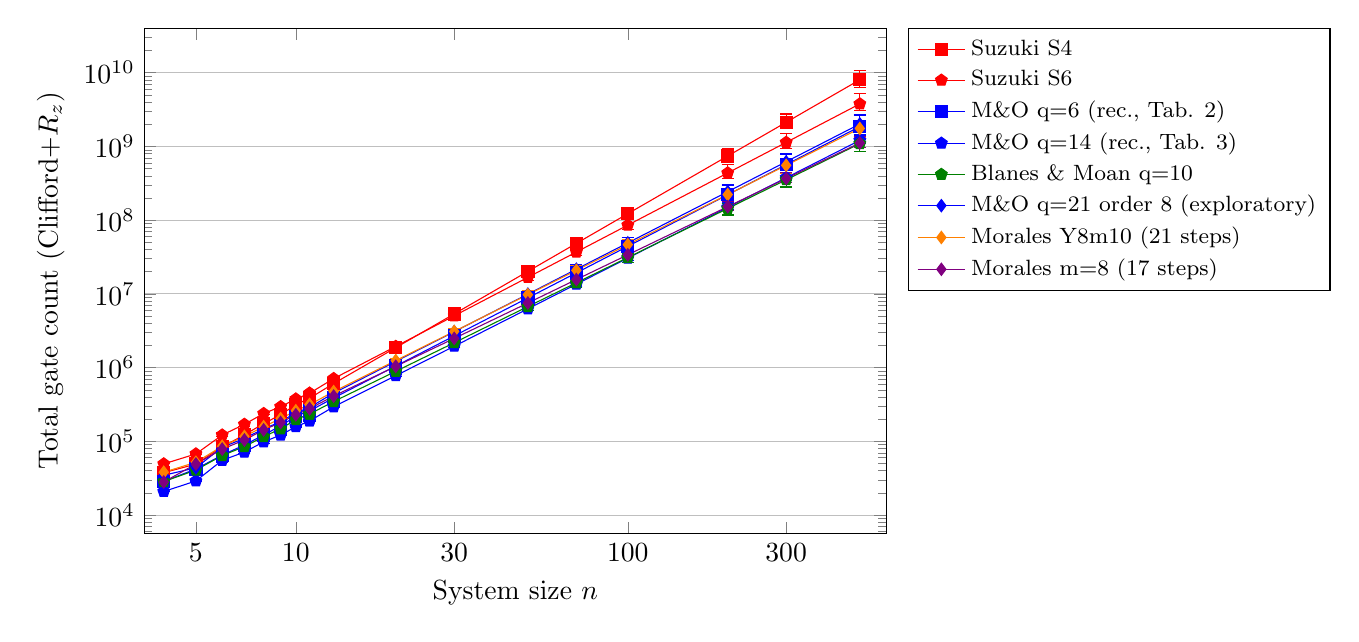
\begin{tikzpicture}
  \begin{loglogaxis}[
    width=11cm, height=8cm,
    xlabel={System size $n$},
    ylabel={Total gate count (Clifford+$R_z$)},
    xtick={5,10,30,100,300}, xticklabels={5,10,30,100,300},
    xmin=3.5, xmax=600,
    ymajorgrids=true,
    legend pos=outer north east,
    legend cell align=left,
    legend style={font=\footnotesize},
  ]
    % suzuki4: measured n, mean over seeds, bars min..max over seeds
    \addplot[red, solid, mark=square*, mark size=2.2pt, mark options={solid, fill=red}, error bars/.cd, y dir=both, y explicit, error bar style={solid}] coordinates {
      (4,37651.2) += (0,508.8) -= (0,339.2)
      (5,49184) += (0,1696) -= (0,1484)
      (6,84333.6) += (0,5978.4) -= (0,4197.6)
      (7,122578) += (0,9497.6) -= (0,8310.4)
      (8,174349) += (0,7123.2) -= (0,6444.8)
      (9,229914) += (0,10494) -= (0,12402)
      (10,315032) += (0,24168) -= (0,11872)
      (11,384780) += (0,16324) -= (0,9328)
    };
    \addlegendentry{Suzuki S4}
    % suzuki4: extrapolated, r = ceil(3.65267 n^1.59931), per step = 212 n + 0; bars min..max of per-seed fits
    \addplot[red, solid, mark=square*, mark size=2.2pt, mark options={solid, fill=red}, forget plot, error bars/.cd, y dir=both, y explicit, error bar style={solid}] coordinates {
      (11,384780)
      (13,609076) += (0,27560) -= (0,19292)
      (20,1.8656e+06) += (0,139920) -= (0,101760)
      (30,5.35512e+06) += (0,553320) -= (0,407040)
      (50,2.0193e+07) += (0,2.9044e+06) -= (0,2.0352e+06)
      (70,4.84229e+07) += (0,8.26588e+06) -= (0,5.66888e+06)
      (100,1.22345e+08) += (0,2.45072e+07) -= (0,1.63664e+07)
      (200,7.41406e+08) += (0,1.92369e+08) -= (0,1.22706e+08)
      (300,2.12697e+09) += (0,6.28432e+08) -= (0,3.9025e+08)
      (500,8.02431e+09) += (0,2.74604e+09) -= (0,1.65e+09)
    };
    % suzuki6: measured n, mean over seeds, bars min..max over seeds
    \addplot[red, solid, mark=pentagon*, mark size=2.2pt, mark options={solid, fill=red}, error bars/.cd, y dir=both, y explicit, error bar style={solid}] coordinates {
      (4,49536) += (0,0) -= (0,0)
      (5,67596) += (0,4644) -= (0,516)
      (6,121982) += (0,8049.6) -= (0,4334.4)
      (7,170486) += (0,10113.6) -= (0,11558.4)
      (8,238598) += (0,9081.6) -= (0,7430.4)
      (9,295358) += (0,11145.6) -= (0,16718.4)
      (10,375648) += (0,26832) -= (0,14448)
      (11,449539) += (0,15892.8) -= (0,6811.2)
    };
    \addlegendentry{Suzuki S6}
    % suzuki6: extrapolated, r = ceil(1.63295 n^1.35284), per step = 1032 n + 0; bars min..max of per-seed fits
    \addplot[red, solid, mark=pentagon*, mark size=2.2pt, mark options={solid, fill=red}, forget plot, error bars/.cd, y dir=both, y explicit, error bar style={solid}] coordinates {
      (11,449539)
      (13,711048) += (0,40248) -= (0,13416)
      (20,1.94016e+06) += (0,165120) -= (0,61920)
      (30,5.04648e+06) += (0,588240) -= (0,278640)
      (50,1.677e+07) += (0,2.7348e+06) -= (0,1.3932e+06)
      (70,3.69869e+07) += (0,7.15176e+06) -= (0,3.68424e+06)
      (100,8.5656e+07) += (0,1.92984e+07) -= (0,1.00104e+07)
      (200,4.37155e+08) += (0,1.28174e+08) -= (0,6.5016e+07)
      (300,1.13499e+09) += (0,3.78641e+08) -= (0,1.89785e+08)
      (500,3.77506e+09) += (0,1.46028e+09) -= (0,7.15692e+08)
    };
    % mo-q6: measured n, mean over seeds, bars min..max over seeds
    \addplot[blue, solid, mark=square*, mark size=2.2pt, mark options={solid, fill=blue}, error bars/.cd, y dir=both, y explicit, error bar style={solid}] coordinates {
      (4,28639.6) += (0,1720.4) -= (0,3339.6)
      (5,42251) += (0,2024) -= (0,4301)
      (6,65122.2) += (0,1669.8) -= (0,2884.2)
      (7,89435.5) += (0,4427.5) -= (0,6198.5)
      (8,122250) += (0,11334.4) -= (0,6881.6)
      (9,162350) += (0,8424.9) -= (0,12068.1)
      (10,219098) += (0,8602) -= (0,14168)
      (11,259376) += (0,27273.4) -= (0,22820.6)
    };
    \addlegendentry{M\&O q=6 (rec., Tab. 2)}
    % mo-q6: extrapolated, r = ceil(3.93927 n^1.32338), per step = 253 n + 0; bars min..max of per-seed fits
    \addplot[blue, solid, mark=square*, mark size=2.2pt, mark options={solid, fill=blue}, forget plot, error bars/.cd, y dir=both, y explicit, error bar style={solid}] coordinates {
      (11,259376)
      (13,388102) += (0,23023) -= (0,16445)
      (20,1.05248e+06) += (0,106260) -= (0,65780)
      (30,2.69445e+06) += (0,371910) -= (0,242880)
      (50,8.8297e+06) += (0,1.63185e+06) -= (0,1.07525e+06)
      (70,1.93039e+07) += (0,4.16185e+06) -= (0,2.72734e+06)
      (100,4.41991e+07) += (0,1.10814e+07) -= (0,7.1599e+06)
      (200,2.21173e+08) += (0,7.09412e+07) -= (0,4.44268e+07)
      (300,5.67352e+08) += (0,2.06296e+08) -= (0,1.26374e+08)
      (500,1.85892e+09) += (0,7.80252e+08) -= (0,4.6337e+08)
    };
    % mo-q14: measured n, mean over seeds, bars min..max over seeds
    \addplot[blue, solid, mark=pentagon*, mark size=2.2pt, mark options={solid, fill=blue}, error bars/.cd, y dir=both, y explicit, error bar style={solid}] coordinates {
      (4,20916) += (0,0) -= (0,0)
      (5,29050) += (0,0) -= (0,0)
      (6,55427.4) += (0,348.6) -= (0,3137.4)
      (7,71579.2) += (0,1626.8) -= (0,2440.2)
      (8,98537.6) += (0,3718.4) -= (0,5577.6)
      (9,121836) += (0,3660.3) -= (0,1568.7)
      (10,158032) += (0,4648) -= (0,1162)
      (11,189174) += (0,2556.4) -= (0,3834.6)
    };
    \addlegendentry{M\&O q=14 (rec., Tab. 3)}
    % mo-q14: extrapolated, r = ceil(1.412 n^1.28559), per step = 581 n + 0; bars min..max of per-seed fits
    \addplot[blue, solid, mark=pentagon*, mark size=2.2pt, mark options={solid, fill=blue}, forget plot, error bars/.cd, y dir=both, y explicit, error bar style={solid}] coordinates {
      (11,189174)
      (13,294567) += (0,0) -= (0,7553)
      (20,778540) += (0,23240) -= (0,23240)
      (30,1.95216e+06) += (0,104580) -= (0,69720)
      (50,6.2748e+06) += (0,464800) -= (0,290500)
      (70,1.35431e+07) += (0,1.2201e+06) -= (0,732060)
      (100,3.06187e+07) += (0,3.2536e+06) -= (0,1.8592e+06)
      (200,1.49085e+08) += (0,2.10322e+07) -= (0,1.08066e+07)
      (300,3.76488e+08) += (0,6.1005e+07) -= (0,3.01539e+07)
      (500,1.21022e+09) += (0,2.27171e+08) -= (0,1.08356e+08)
    };
    % bm-q10: measured n, mean over seeds, bars min..max over seeds
    \addplot[green!50!black, solid, mark=pentagon*, mark size=2.2pt, mark options={solid, fill=green!50!black}, error bars/.cd, y dir=both, y explicit, error bar style={solid}] coordinates {
      (4,28522.8) += (0,1501.2) -= (0,166.8)
      (5,40866) += (0,834) -= (0,1251)
      (6,64301.4) += (0,750.6) -= (0,1751.4)
      (7,84942.9) += (0,2627.1) -= (0,3210.9)
      (8,116093) += (0,7339.2) -= (0,6004.8)
      (9,148244) += (0,5629.5) -= (0,9382.5)
      (10,197658) += (0,2502) -= (0,5838)
      (11,234854) += (0,12843.6) -= (0,10091.4)
    };
    \addlegendentry{Blanes \& Moan q=10}
    % bm-q10: extrapolated, r = ceil(2.82314 n^1.2111), per step = 417 n + 0; bars min..max of per-seed fits
    \addplot[green!50!black, solid, mark=pentagon*, mark size=2.2pt, mark options={solid, fill=green!50!black}, forget plot, error bars/.cd, y dir=both, y explicit, error bar style={solid}] coordinates {
      (11,234854)
      (13,346944) += (0,5421) -= (0,10842)
      (20,892380) += (0,33360) -= (0,50040)
      (30,2.17674e+06) += (0,137610) -= (0,175140)
      (50,6.73455e+06) += (0,625500) -= (0,729750)
      (70,1.41572e+07) += (0,1.57626e+06) -= (0,1.80978e+06)
      (100,3.11499e+07) += (0,4.1283e+06) -= (0,4.587e+06)
      (200,1.44115e+08) += (0,2.53536e+07) -= (0,2.63544e+07)
      (300,3.53282e+08) += (0,7.09317e+07) -= (0,7.18074e+07)
      (500,1.09296e+09) += (0,2.55204e+08) -= (0,2.49366e+08)
    };
    % mo-o8-q21: measured n, mean over seeds, bars min..max over seeds
    \addplot[blue, solid, mark=diamond*, mark size=2.2pt, mark options={solid, fill=blue}, error bars/.cd, y dir=both, y explicit, error bar style={solid}] coordinates {
      (4,34720) += (0,0) -= (0,0)
      (5,43834) += (0,3906) -= (0,434)
      (6,83328) += (0,5208) -= (0,5208)
      (7,109976) += (0,5468.4) -= (0,6683.6)
      (8,147907) += (0,4860.8) -= (0,9027.2)
      (9,185144) += (0,2343.6) -= (0,5468.4)
      (10,243908) += (0,16492) -= (0,9548)
      (11,289304) += (0,6683.6) -= (0,2864.4)
    };
    \addlegendentry{M\&O q=21 order 8 (exploratory)}
    % mo-o8-q21: extrapolated, r = ceil(1.3736 n^1.30758), per step = 868 n + 0; bars min..max of per-seed fits
    \addplot[blue, solid, mark=diamond*, mark size=2.2pt, mark options={solid, fill=blue}, forget plot, error bars/.cd, y dir=both, y explicit, error bar style={solid}] coordinates {
      (11,289304)
      (13,451360) += (0,11284) -= (0,11284)
      (20,1.2152e+06) += (0,69440) -= (0,52080)
      (30,3.07272e+06) += (0,260400) -= (0,182280)
      (50,9.9386e+06) += (0,1.302e+06) -= (0,868000)
      (70,2.16306e+07) += (0,3.40256e+06) -= (0,2.30888e+06)
      (100,4.92156e+07) += (0,9.2876e+06) -= (0,6.2496e+06)
      (200,2.43387e+08) += (0,6.076e+07) -= (0,3.95808e+07)
      (300,6.20273e+08) += (0,1.77853e+08) -= (0,1.13274e+08)
      (500,2.01593e+09) += (0,6.75304e+08) -= (0,4.19244e+08)
    };
    % morales-y8m10: measured n, mean over seeds, bars min..max over seeds
    \addplot[orange, solid, mark=diamond*, mark size=2.2pt, mark options={solid, fill=orange}, error bars/.cd, y dir=both, y explicit, error bar style={solid}] coordinates {
      (4,38192) += (0,0) -= (0,0)
      (5,52080) += (0,0) -= (0,0)
      (6,85932) += (0,2604) -= (0,2604)
      (7,116659) += (0,4860.8) -= (0,1215.2)
      (8,158323) += (0,8332.8) -= (0,5555.2)
      (9,203893) += (0,7030.8) -= (0,8593.2)
      (10,260400) += (0,17360) -= (0,8680)
      (11,315084) += (0,9548) -= (0,9548)
    };
    \addlegendentry{Morales Y8m10 (21 steps)}
    % morales-y8m10: extrapolated, r = ceil(1.66328 n^1.25438), per step = 868 n + 0; bars min..max of per-seed fits
    \addplot[orange, solid, mark=diamond*, mark size=2.2pt, mark options={solid, fill=orange}, forget plot, error bars/.cd, y dir=both, y explicit, error bar style={solid}] coordinates {
      (11,315084)
      (13,473928) += (0,11284) -= (0,22568)
      (20,1.24992e+06) += (0,69440) -= (0,86800)
      (30,3.09876e+06) += (0,286440) -= (0,286440)
      (50,9.765e+06) += (0,1.2152e+06) -= (0,1.2152e+06)
      (70,2.09014e+07) += (0,3.038e+06) -= (0,3.038e+06)
      (100,4.66116e+07) += (0,8.0724e+06) -= (0,7.7252e+06)
      (200,2.22382e+08) += (0,4.98232e+07) -= (0,4.54832e+07)
      (300,5.54652e+08) += (0,1.41397e+08) -= (0,1.25513e+08)
      (500,1.75423e+09) += (0,5.17328e+08) -= (0,4.43982e+08)
    };
    % morales-m8: measured n, mean over seeds, bars min..max over seeds
    \addplot[violet, solid, mark=diamond*, mark size=2.2pt, mark options={solid, fill=violet}, error bars/.cd, y dir=both, y explicit, error bar style={solid}] coordinates {
      (4,28160) += (0,0) -= (0,0)
      (5,49280) += (0,0) -= (0,0)
      (6,78566.4) += (0,1689.6) -= (0,2534.4)
      (7,104474) += (0,3942.4) -= (0,985.6)
      (8,143053) += (0,9011.2) -= (0,2252.8)
      (9,180576) += (0,3168) -= (0,3168)
      (10,229504) += (0,9856) -= (0,4224)
      (11,278010) += (0,8518.4) -= (0,6969.6)
    };
    \addlegendentry{Morales m=8 (17 steps)}
    % morales-m8: extrapolated, r = ceil(2.19247 n^1.17079), per step = 704 n + 0; bars min..max of per-seed fits
    \addplot[violet, solid, mark=diamond*, mark size=2.2pt, mark options={solid, fill=violet}, forget plot, error bars/.cd, y dir=both, y explicit, error bar style={solid}] coordinates {
      (11,278010)
      (13,411840) += (0,9152) -= (0,9152)
      (20,1.04192e+06) += (0,42240) -= (0,42240)
      (30,2.49216e+06) += (0,168960) -= (0,126720)
      (50,7.5328e+06) += (0,739200) -= (0,492800)
      (70,1.5671e+07) += (0,1.7248e+06) -= (0,1.18272e+06)
      (100,3.39328e+07) += (0,4.5056e+06) -= (0,2.9568e+06)
      (200,1.52627e+08) += (0,2.61888e+07) -= (0,1.63328e+07)
      (300,3.68122e+08) += (0,7.13856e+07) -= (0,4.39296e+07)
      (500,1.11549e+09) += (0,2.4992e+08) -= (0,1.496e+08)
    };
  \end{loglogaxis}
\end{tikzpicture}
